% ============================
% DOCUMENT SETUP
% ============================
\documentclass[12pt]{article}

% ============================
% PACKAGES
% ============================

% --- Matemáticas ---
\usepackage{amsmath, amsthm, amssymb, amsfonts, amsbsy, amscd}

% --- Tablas y Figuras ---
\usepackage{graphicx} % Para incluir imágenes
\usepackage{tabularx} % Tablas de ancho automático
\usepackage{float}    % Mejor control de ubicación de figuras/tablas
\usepackage{booktabs} % Mejor estilo para tablas
\usepackage{multirow} % Combinar filas en tablas
\usepackage{diagbox}  % Crear diagonales en tablas
\usepackage{subfig}   % Subfiguras
\usepackage{caption}  % Personalizar leyendas

% --- Tipografía y Formato ---
\usepackage{times}       % Fuente Times New Roman
\usepackage{setspace}    % Espaciado
\usepackage{microtype}   % Mejoras tipográficas
\usepackage[none]{hyphenat} % Evitar partición de palabras

% --- Geometría ---
\usepackage[letterpaper, bottom=2.5cm, top=2.5cm, right=2.5cm, left=3cm, headsep=1.5cm]{geometry}

% --- Encabezados y Pies de Página ---
\usepackage{fancyhdr}
\usepackage{lastpage}

% --- Enumeraciones ---
\usepackage{enumitem} % Mejor control sobre listas

% --- Otros ---
\usepackage{tikz}     % Para gráficos vectoriales
\usepackage{cancel}   % Para tachar en fórmulas
\usepackage{cite}     % Para manejo de citas
\usepackage{chicago}  % Estilo de bibliografía Chicago

% --- Enlaces e Hipervínculos ---
\usepackage{hyperref}
\hypersetup{
    colorlinks=true,
    breaklinks=true,
    linkcolor=black,
    citecolor=blue,
    filecolor=magenta,
    urlcolor=blue
}

% ============================
% DEFINICIONES
% ============================

\providecommand{\abs}[1]{\lvert#1\rvert}

\DeclareMathOperator*{\argmin}{arg\,min} % Operador argmin
\DeclareMathOperator*{\argmax}{arg\,max} % Operador argmax

\renewcommand*\contentsname{Index} % Cambiar nombre de tabla de contenidos
\setlength{\footskip}{45pt} % Distancia pie de página
\setlength{\parindent}{0pt} % Sin sangría en párrafos

% ============================
% DOCUMENTO
% ============================

\title{\textbf{Homework 2, Final Report\\ \vspace{0.5cm} \\ Finite Elements}}
\def\footerlogo{LOGO_UNIVERSIDAD.jpg} % Logo para el pie de página
\date{\textbf{April 25, 2025}}

\begin{document}
\makeatletter
\begin{titlepage}
    \begin{center}
        \vspace{2cm}
        
\includegraphics[width=0.8\linewidth]{LOGO_UNIVERSIDAD.jpg}\\[10ex]
        
        \rule{\textwidth}{1pt} \\[2ex]
        {\LARGE \textbf{Homework 2, Final Report\\ \vspace{0.5cm} Finite Elements}}\\[2ex]
        \rule{\textwidth}{1pt} \\[10ex]

        \vfill

        \begin{flushright}
            \textbf{Professor:\\
             Jose A. Abell} \\[0.3cm]
            \textbf{Students: \\
            Bernardo Caprile\\
            Pedro Valenzuela} \\[0.3cm]
        \end{flushright}
        
        \vspace*{1cm}
        {\normalsize \@date}
    \end{center}
\end{titlepage}
\makeatother


\pagestyle{fancy}
\fancyhf{}
\rhead{\shorttitle}


%\lhead{Guides and tutorials}
\rfoot{\thepage}
\lhead{Finite Elements} 
\rhead{
\includegraphics[width=0.25\linewidth]{LOGO_UNIVERSIDAD.jpg}} % For header of the document
\renewcommand{\footrulewidth}{0.5pt}

\tableofcontents

%% If you write a long report, add list of figures and tables and start reporting on new page
%\listoffigures
%\listoftables
%\newpage
\thispagestyle{empty}
\newpage
\spacing{1.15}
\setcounter{page}{1}

\section{Introduction}

This project analyzes the mechanical response of a 3D-printed PLA wrench under different loading conditions using the finite element method (FEM).

The goal is to determine the distribution of stress and strain fields, observe the deformation behavior, and identify potential failure regions based on material properties.  
Three loading scenarios are considered: distributed load, point load, and distributed load including the self-weight of the wrench.

The study includes a mesh convergence analysis to ensure the reliability of the results and applies smoothing techniques to improve the visualization of stress and strain fields.  
The results are interpreted using principal stresses and strains, which provide a clearer understanding of critical zones under different loading conditions.

\newpage

\section{Summary of Main Theoretical Points}

The generation of the presented results is based on the fundamental principles of continum mechanics and the finite element method (FEM).

In this analysis, the wrench is modeled as a continuous and elastic solid material subjected to external forces and self-weight.  
The stress components ($\sigma_{xx}$, $\sigma_{yy}$, $\sigma_{xy}$) and strain components ($\epsilon_{xx}$, $\epsilon_{yy}$, $\epsilon_{xy}$) are derived from the linear theory of elasticity, assuming small deformations and material isotropy.

The finite element method is used to discretize the geometry into small elements, solving the equilibrium equations numerically to obtain the fields of displacements, stresses, and strains.  
Convergence studies are performed to ensure that the numerical results are independent of the mesh size, and smoothing techniques are applied to reduce numerical noise and improve the quality of the stress and strain fields.

Principal stresses and strains are computed from the stress and strain tensors to better interpret the mechanical response and predict failure under critical loading conditions.

\section{PLA Material Properties}
The wrench analyzed in this study is 3D-printed using Polylactic Acid (PLA), a thermoplastic polymer derived from renewable resources such as corn starch or sugarcane.

For the mechanical analysis, the following typical material properties were considered based on available data:  
a density between 1210 and 1430 kg/m\textsuperscript{3} (a representative value of 1250 kg/m\textsuperscript{3} was adopted),  
a Young's modulus of approximately 2.7 GPa,  
and a tensile strength in the range of 50 to 70 MPa, with a conservative value of 50 MPa used for failure evaluation. (Wikipedia contributors, no date)

These properties correspond to general values reported for PLA and may vary depending on specific formulation and manufacturing conditions.  
It is also noted that mechanical properties can significantly change based on printing parameters such as orientation, temperature, and layer thickness, as highlighted in the consulted reference.


\newpage
\section{Results}

\subsection{Case 1}

The first case corresponds to the situation where the total load of 30 kgf is applied as a distributed force along the nodes located at the wrench's end.  
The results obtained include the stress and strain components ($\sigma_{xx}$, $\sigma_{yy}$, $\sigma_{xy}$, $\epsilon_{xx}$, $\epsilon_{yy}$, $\epsilon_{xy}$), as well as the principal stress and strain components ($\sigma_1$, $\sigma_2$, $\epsilon_1$, $\epsilon_2$).

The filled contour plots show the distribution of stresses and strains across the geometry. Smoothing has been applied to the results to improve visualization and facilitate the interpretation of stress and strain gradients.  
It is observed that the maximum principal stress $\sigma_1$ occurs near the inner corner of the wrench, where stress concentration is expected, while the minimum principal stress $\sigma_2$ is distributed along the outer surfaces.


\begin{figure}[H]
    \centering
    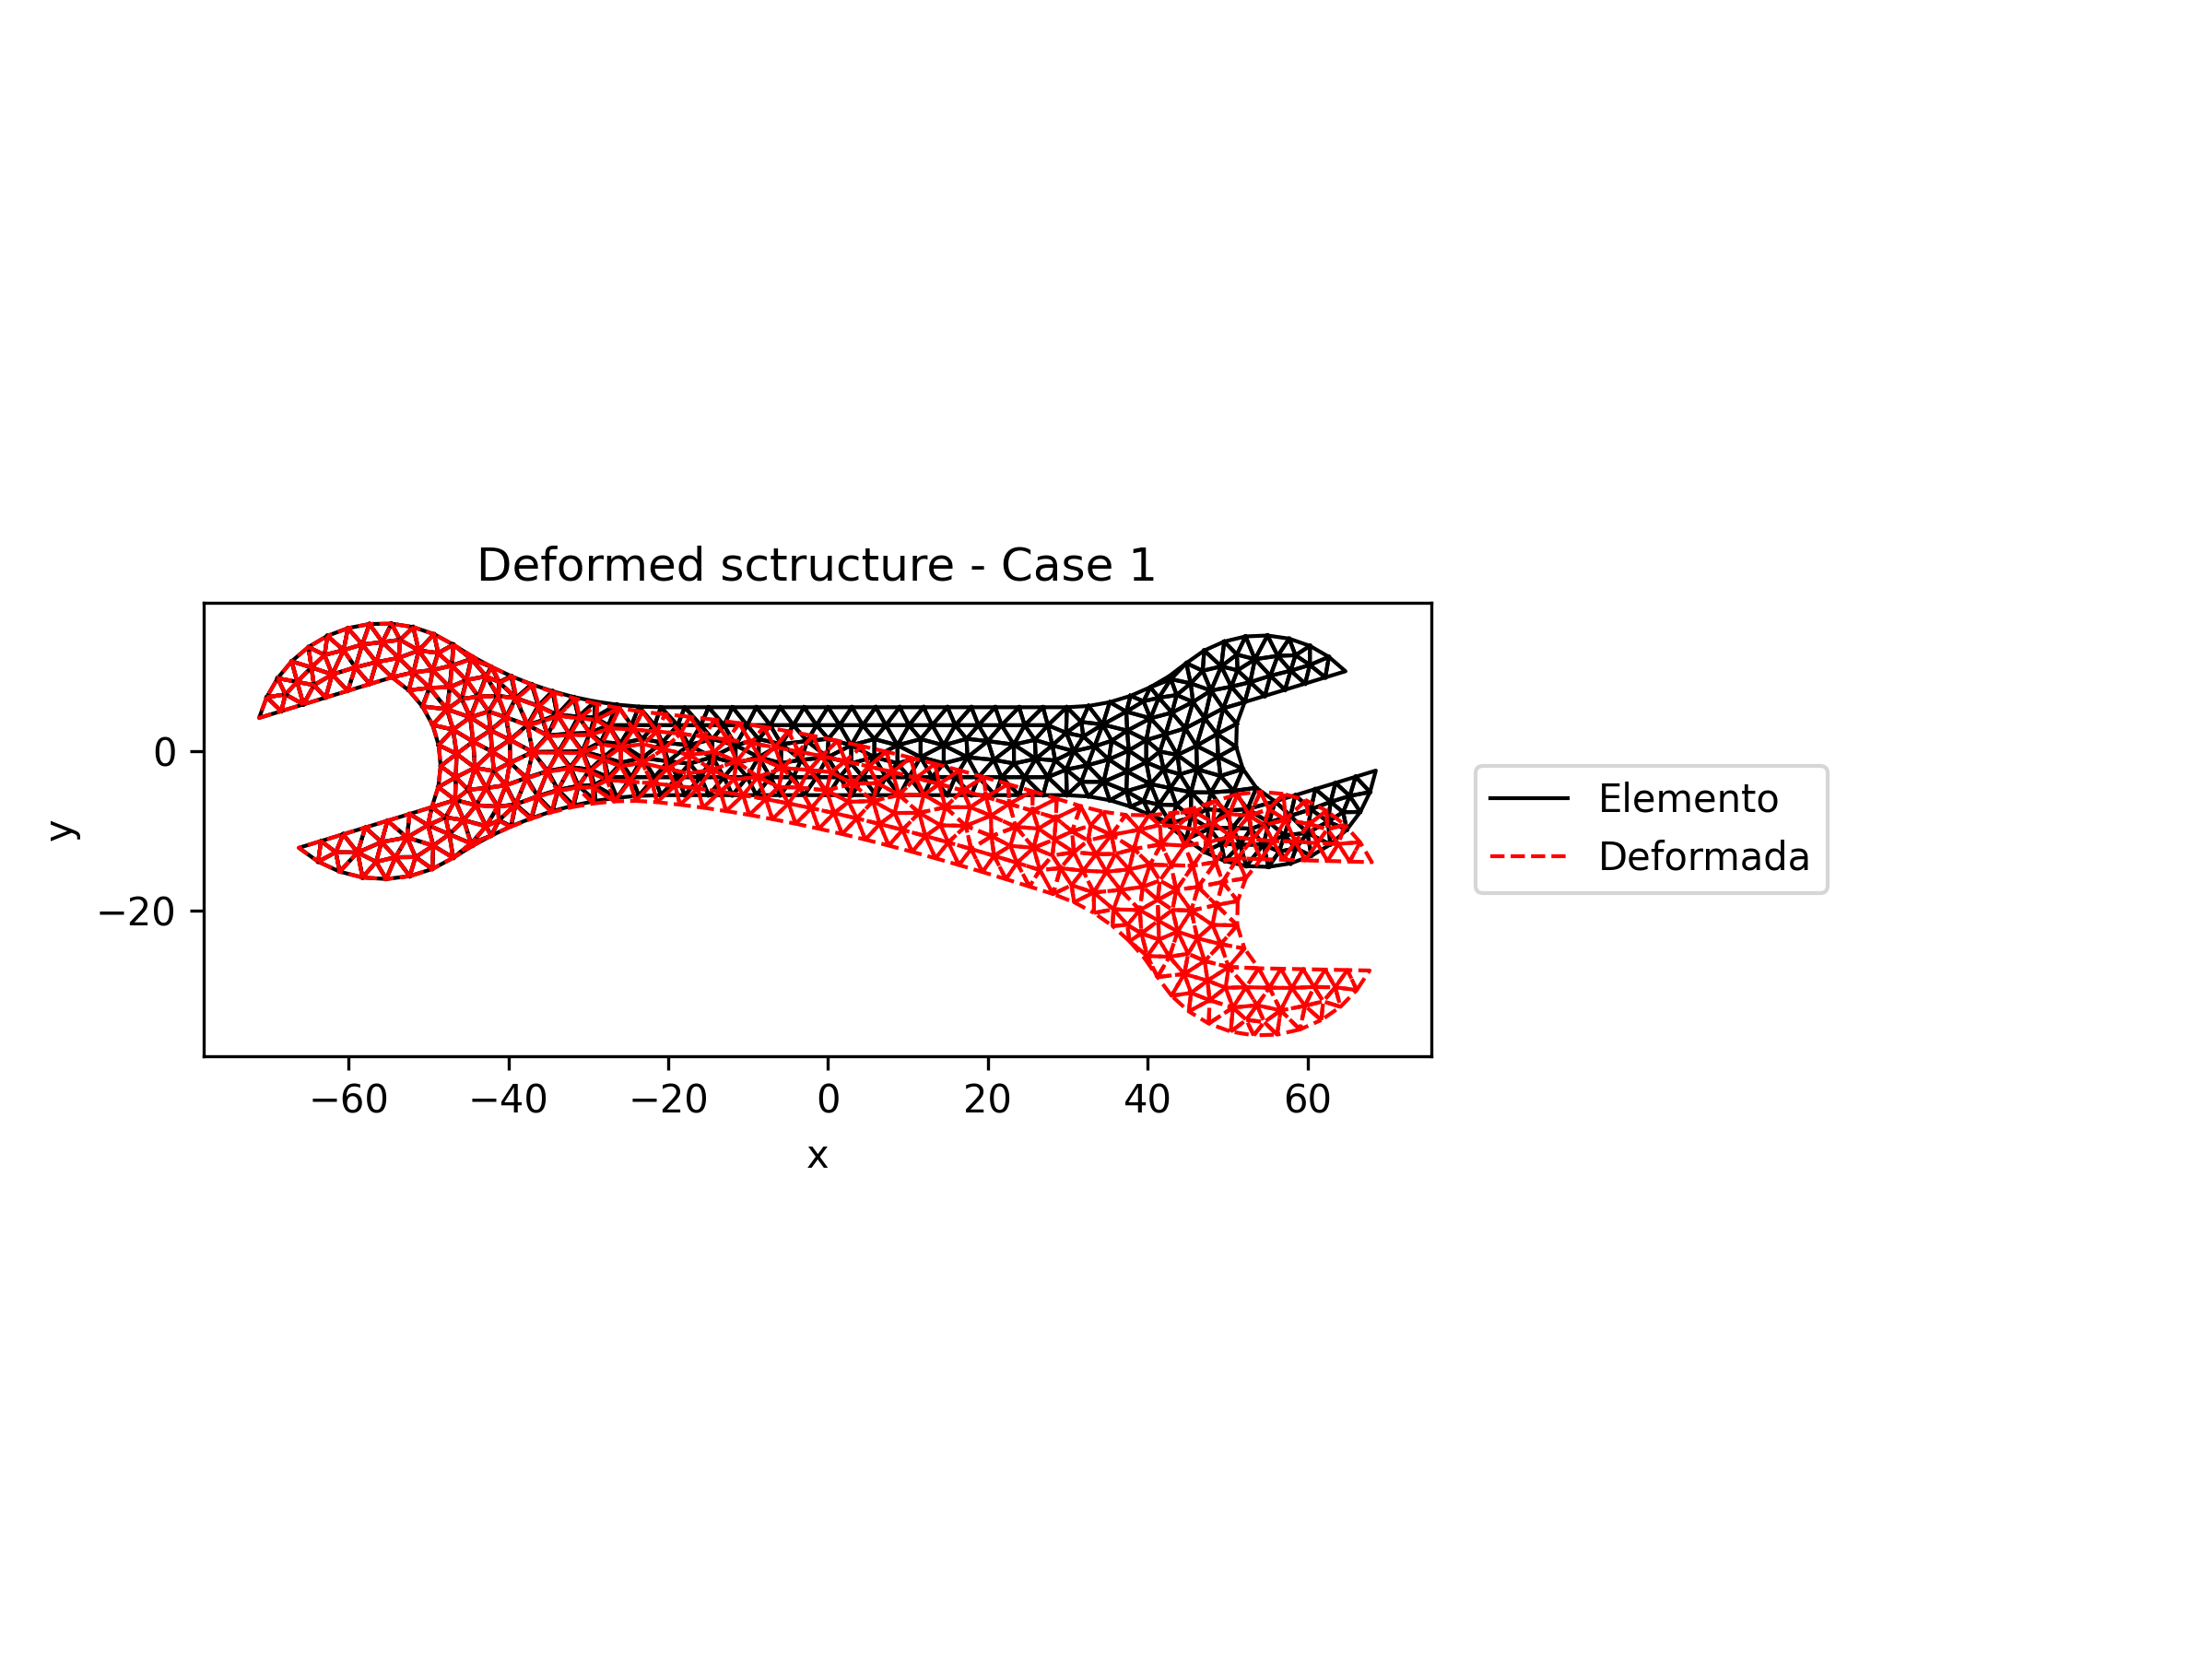
\includegraphics[width=0.8\textwidth]{Resultados/Deformed_sctructure_-_Case_1.png}
    \caption{Deformed structure - Case 1}
    \label{fig:fig1}
\end{figure}

\begin{figure}[H]
    \centering
    \begin{minipage}{0.48\textwidth}
        \centering
        \includegraphics[width=\textwidth]{Resultados/Case_1_-_Maximum_Principal_Stress_σ1.png}
        \caption{Maximum Principal Stress $\sigma_1$}
        \label{fig:fig2}
    \end{minipage}
    \hfill
    \begin{minipage}{0.48\textwidth}
        \centering
        \includegraphics[width=\textwidth]{Resultados/Case_1_-_Minimum_Principal_Strain_ε2.png}
        \caption{Minimum Principal Strain $\epsilon_2$}
        \label{fig:fig3}
    \end{minipage}
\end{figure}

\begin{figure}[H]
    \centering
    \begin{minipage}{0.48\textwidth}
        \centering
        \includegraphics[width=\textwidth]{Resultados/Case_1_-_Strain_εxx.png}
        \caption{Strain $\epsilon_{xx}$}
        \label{fig:fig4}
    \end{minipage}
    \hfill
    \begin{minipage}{0.48\textwidth}
        \centering
        \includegraphics[width=\textwidth]{Resultados/Case_1_-_Strain_εxy.png}
        \caption{Strain $\epsilon_{xy}$}
        \label{fig:fig5}
    \end{minipage}
\end{figure}

\begin{figure}[H]
    \centering
    \begin{minipage}{0.48\textwidth}
        \centering
        \includegraphics[width=\textwidth]{Resultados/Case_1_-_Strain_εyy.png}
        \caption{Strain $\epsilon_{yy}$}
        \label{fig:fig6}
    \end{minipage}
    \hfill
    \begin{minipage}{0.48\textwidth}
        \centering
        \includegraphics[width=\textwidth]{Resultados/Case_1_-_Maximum_Principal_Strain_ε1.png}
        \caption{Maximum Principal Strain $\epsilon_1$}
        \label{fig:fig7}
    \end{minipage}
\end{figure}

\begin{figure}[H]
    \centering
    \begin{minipage}{0.48\textwidth}
        \centering
        \includegraphics[width=\textwidth]{Resultados/Case_1_-_Minimum_Principal_Stress_σ2.png}
        \caption{Minimum Principal Stress $\sigma_2$}
        \label{fig:fig8}
    \end{minipage}
    \hfill
    \begin{minipage}{0.48\textwidth}
        \centering
        \includegraphics[width=\textwidth]{Resultados/Case_1_-_Stress_σxx.png}
        \caption{Stress $\sigma_{xx}$}
        \label{fig:fig9}
    \end{minipage}
\end{figure}

\begin{figure}[H]
    \centering
    \begin{minipage}{0.48\textwidth}
        \centering
        \includegraphics[width=\textwidth]{Resultados/Case_1_-_Stress_σxy.png}
        \caption{Stress $\sigma_{xy}$}
        \label{fig:fig10}
    \end{minipage}
    \hfill
    \begin{minipage}{0.48\textwidth}
        \centering
        \includegraphics[width=\textwidth]{Resultados/Case_2_-_Stress_σyy.png}
        \caption{Stress $\sigma_{yy}$}
        \label{fig:fig11}
    \end{minipage}
\end{figure}

\newpage

\subsection{Case 2}

In the second case, the same total load of 30 kgf is applied, but now concentrated at a single node at the end of the wrench.  
This setup simulates an extreme point load condition, increasing local stresses compared to the distributed load case.

As shown in the plots, the maximum principal stresses and strains are much more localized and of greater magnitude around the loaded node.  
The fields $\sigma_{xx}$, $\sigma_{yy}$, and $\sigma_{xy}$ clearly reveal this effect, with very sharp gradients near the application point.  
Similarly, the strains $\epsilon_{xx}$, $\epsilon_{yy}$, and $\epsilon_{xy}$ highlight localized deformations that are more intense compared to Case 1.

\begin{figure}[H]
    \centering
    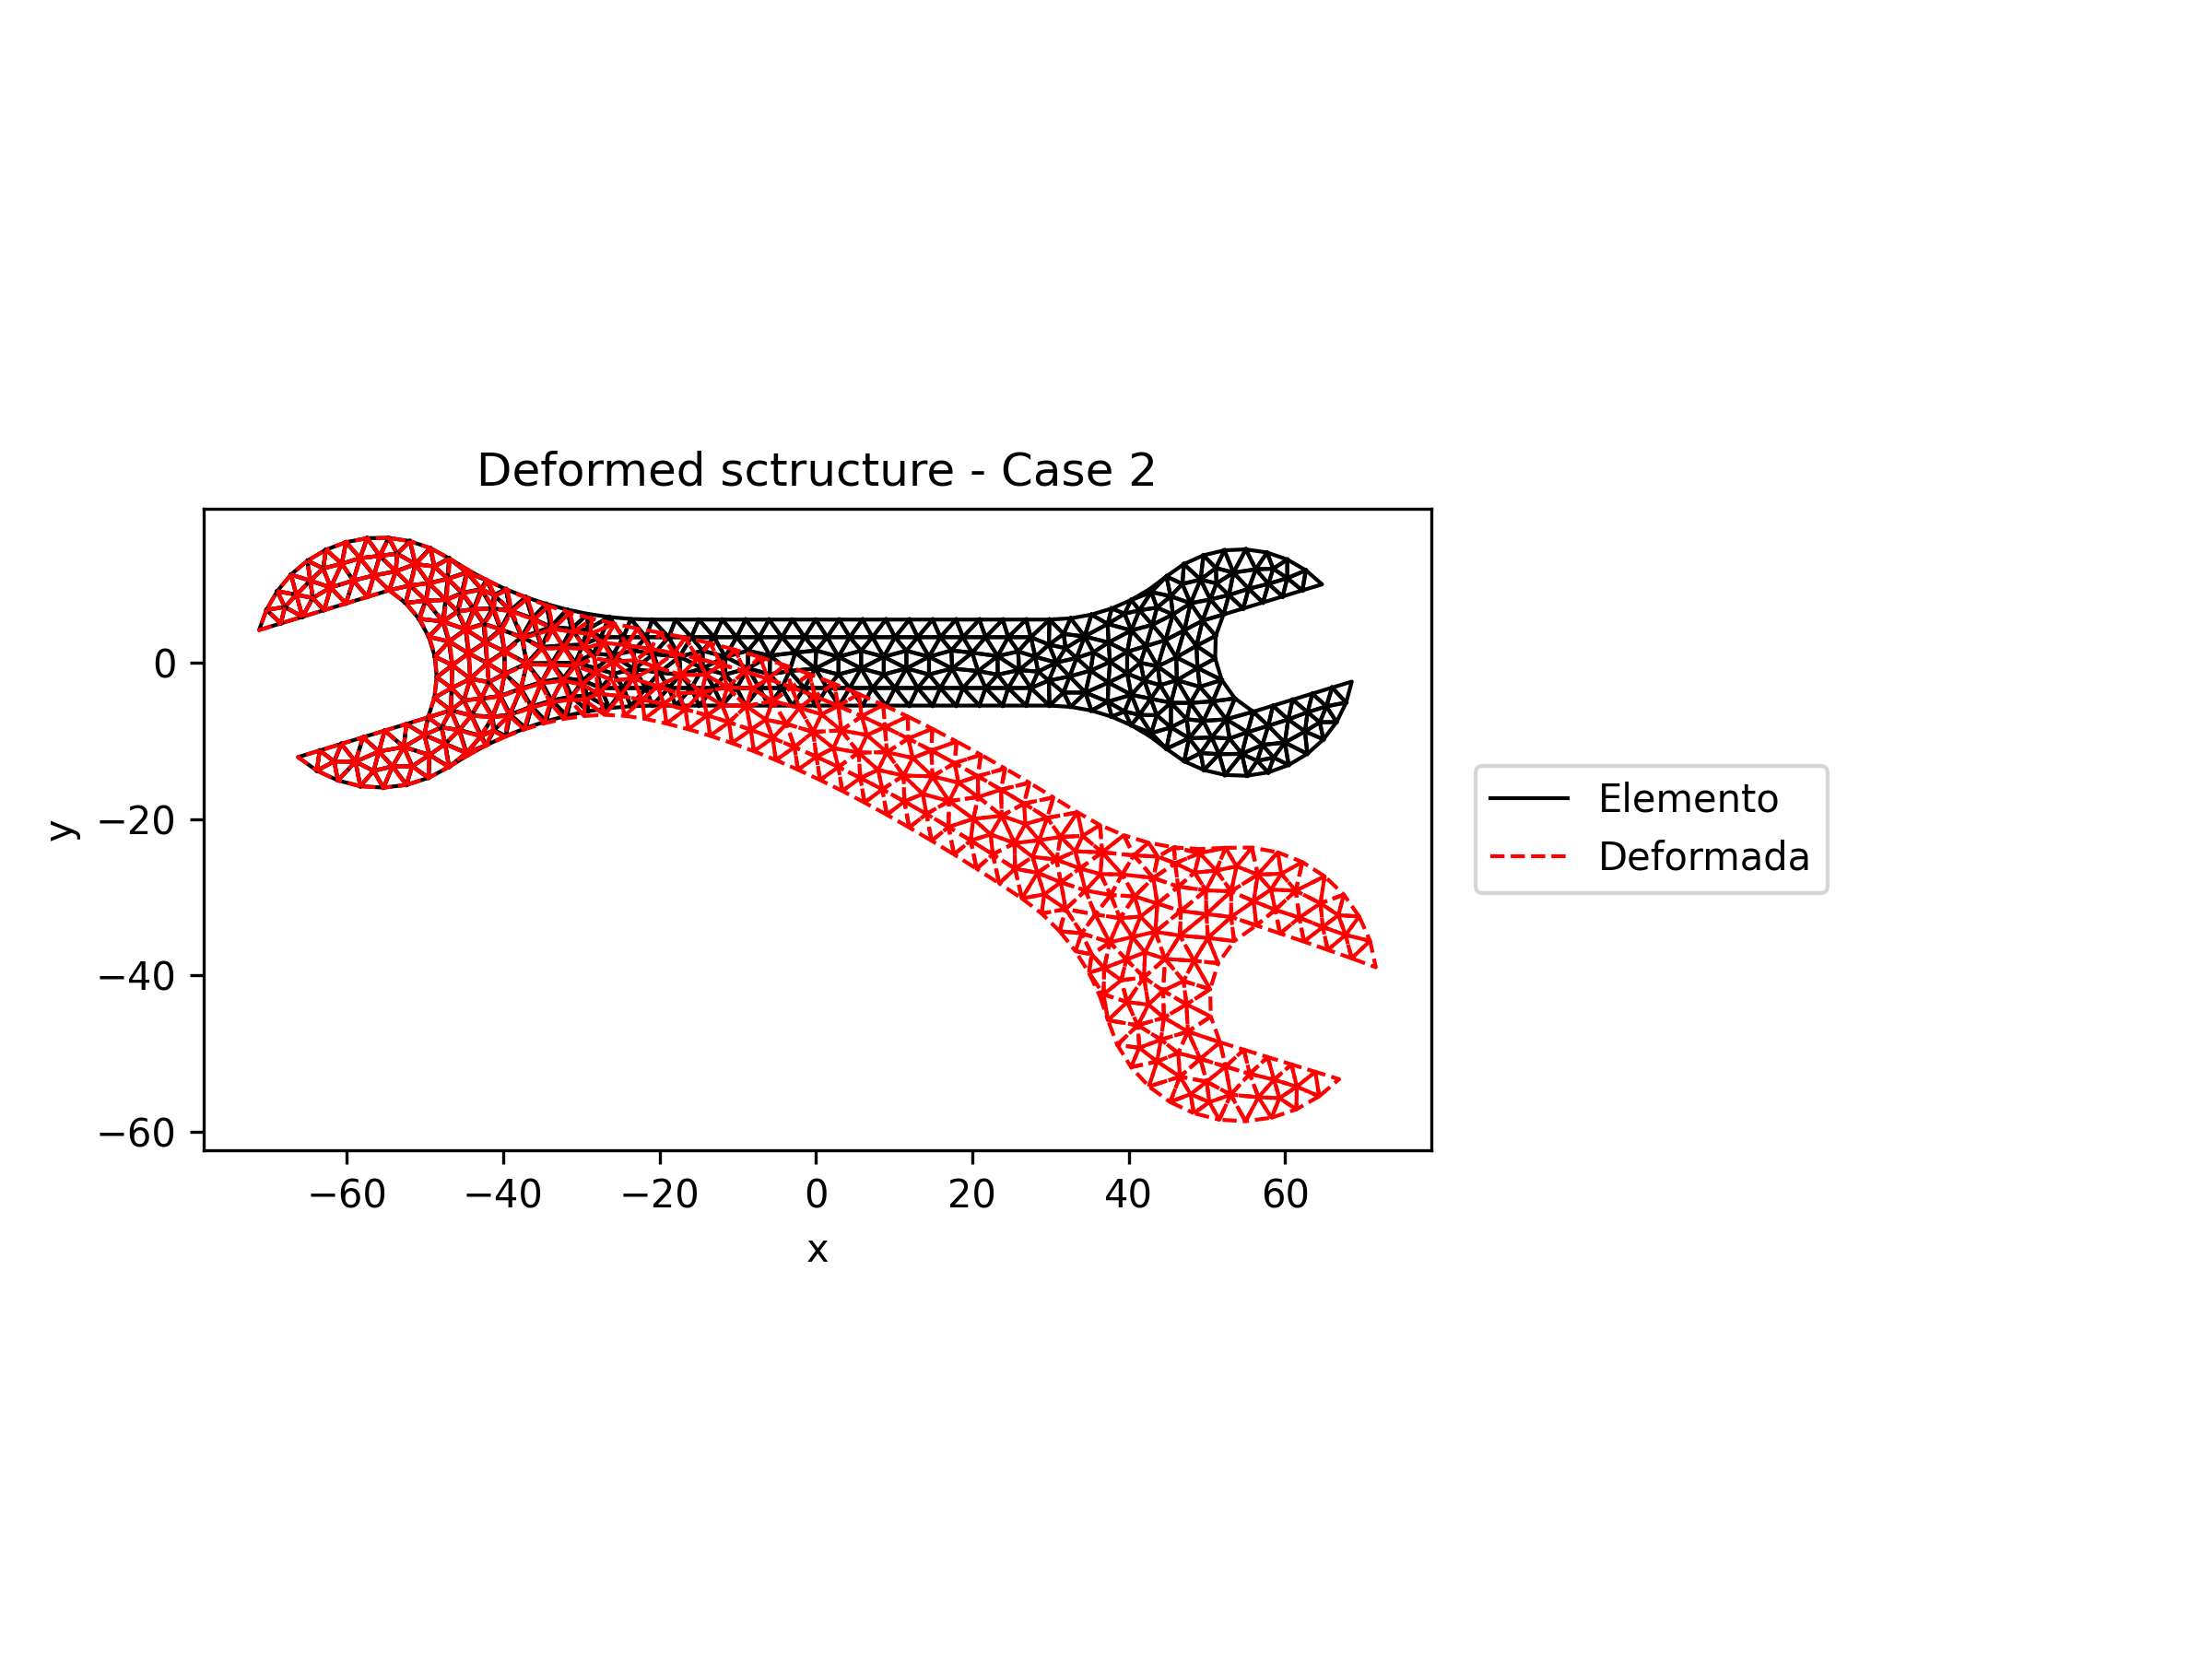
\includegraphics[width=0.8\textwidth]{Resultados/Deformed_sctructure_-_Case_2.png}
    \caption{Deformed structure - Case 2}
    \label{fig:fig12}
\end{figure}

% Imágenes de a dos:
\begin{figure}[H]
    \centering
    \begin{minipage}{0.48\textwidth}
        \centering
        \includegraphics[width=\textwidth]{Resultados/Case_2_-_Maximum_Principal_Stress_σ1.png}
        \caption{Maximum Principal Stress $\sigma_1$}
        \label{fig:fig13}
    \end{minipage}
    \hfill
    \begin{minipage}{0.48\textwidth}
        \centering
        \includegraphics[width=\textwidth]{Resultados/Case_2_-_Minimum_Principal_Strain_ε2.png}
        \caption{Minimum Principal Strain $\epsilon_2$}
        \label{fig:fig14}
    \end{minipage}
\end{figure}

\begin{figure}[H]
    \centering
    \begin{minipage}{0.48\textwidth}
        \centering
        \includegraphics[width=\textwidth]{Resultados/Case_2_-_Strain_εxx.png}
        \caption{Strain $\epsilon_{xx}$}
        \label{fig:fig15}
    \end{minipage}
    \hfill
    \begin{minipage}{0.48\textwidth}
        \centering
        \includegraphics[width=\textwidth]{Resultados/Case_2_-_Strain_εxy.png}
        \caption{Strain $\epsilon_{xy}$}
        \label{fig:fig16}
    \end{minipage}
\end{figure}

\begin{figure}[H]
    \centering
    \begin{minipage}{0.48\textwidth}
        \centering
        \includegraphics[width=\textwidth]{Resultados/Case_2_-_Strain_εyy.png}
        \caption{Strain $\epsilon_{yy}$}
        \label{fig:fig17}
    \end{minipage}
    \hfill
    \begin{minipage}{0.48\textwidth}
        \centering
        \includegraphics[width=\textwidth]{Resultados/Case_2_-_Maximum_Principal_Strain_ε1.png}
        \caption{Maximum Principal Strain $\epsilon_1$}
        \label{fig:fig18}
    \end{minipage}
\end{figure}

\begin{figure}[H]
    \centering
    \begin{minipage}{0.48\textwidth}
        \centering
        \includegraphics[width=\textwidth]{Resultados/Case_2_-_Minimum_Principal_Stress_σ2.png}
        \caption{Minimum Principal Stress $\sigma_2$}
        \label{fig:fig19}
    \end{minipage}
    \hfill
    \begin{minipage}{0.48\textwidth}
        \centering
        \includegraphics[width=\textwidth]{Resultados/Case_2_-_Stress_σxx.png}
        \caption{Stress $\sigma_{xx}$}
        \label{fig:fig20}
    \end{minipage}
\end{figure}

\begin{figure}[H]
    \centering
    \begin{minipage}{0.48\textwidth}
        \centering
        \includegraphics[width=\textwidth]{Resultados/Case_1_-_Stress_σxy.png}
        \caption{Stress $\sigma_{xy}$}
        \label{fig:fig21}
    \end{minipage}
    \hfill
    \begin{minipage}{0.48\textwidth}
        \centering
        \includegraphics[width=\textwidth]{Resultados/Case_1_-_Stress_σyy.png}
        \caption{Stress $\sigma_{yy}$}
        \label{fig:fig22}
    \end{minipage}
\end{figure}



\newpage
\subsection{Case 3}

The third case considers the distributed 30 kgf load along with the self-weight of the wrench itself, modeled as a uniformly distributed gravitational body force.

The results illustrate that the inclusion of self-weight slightly increases the stress and strain levels across the structure, particularly towards the free end of the wrench where both the external load and the accumulated self-weight act together.

While the qualitative patterns of stress and strain are similar to those in Case 1, the values are somewhat higher.  
This shows that for accurate simulations of larger or heavier tools, it becomes important to consider self-weight effects.

The deformation and stress distribution plots confirm that areas of maximum stress and strain are consistent with those previously observed, but magnitudes are marginally larger due to the additional body force contribution.

\begin{figure}[H]
    \centering
    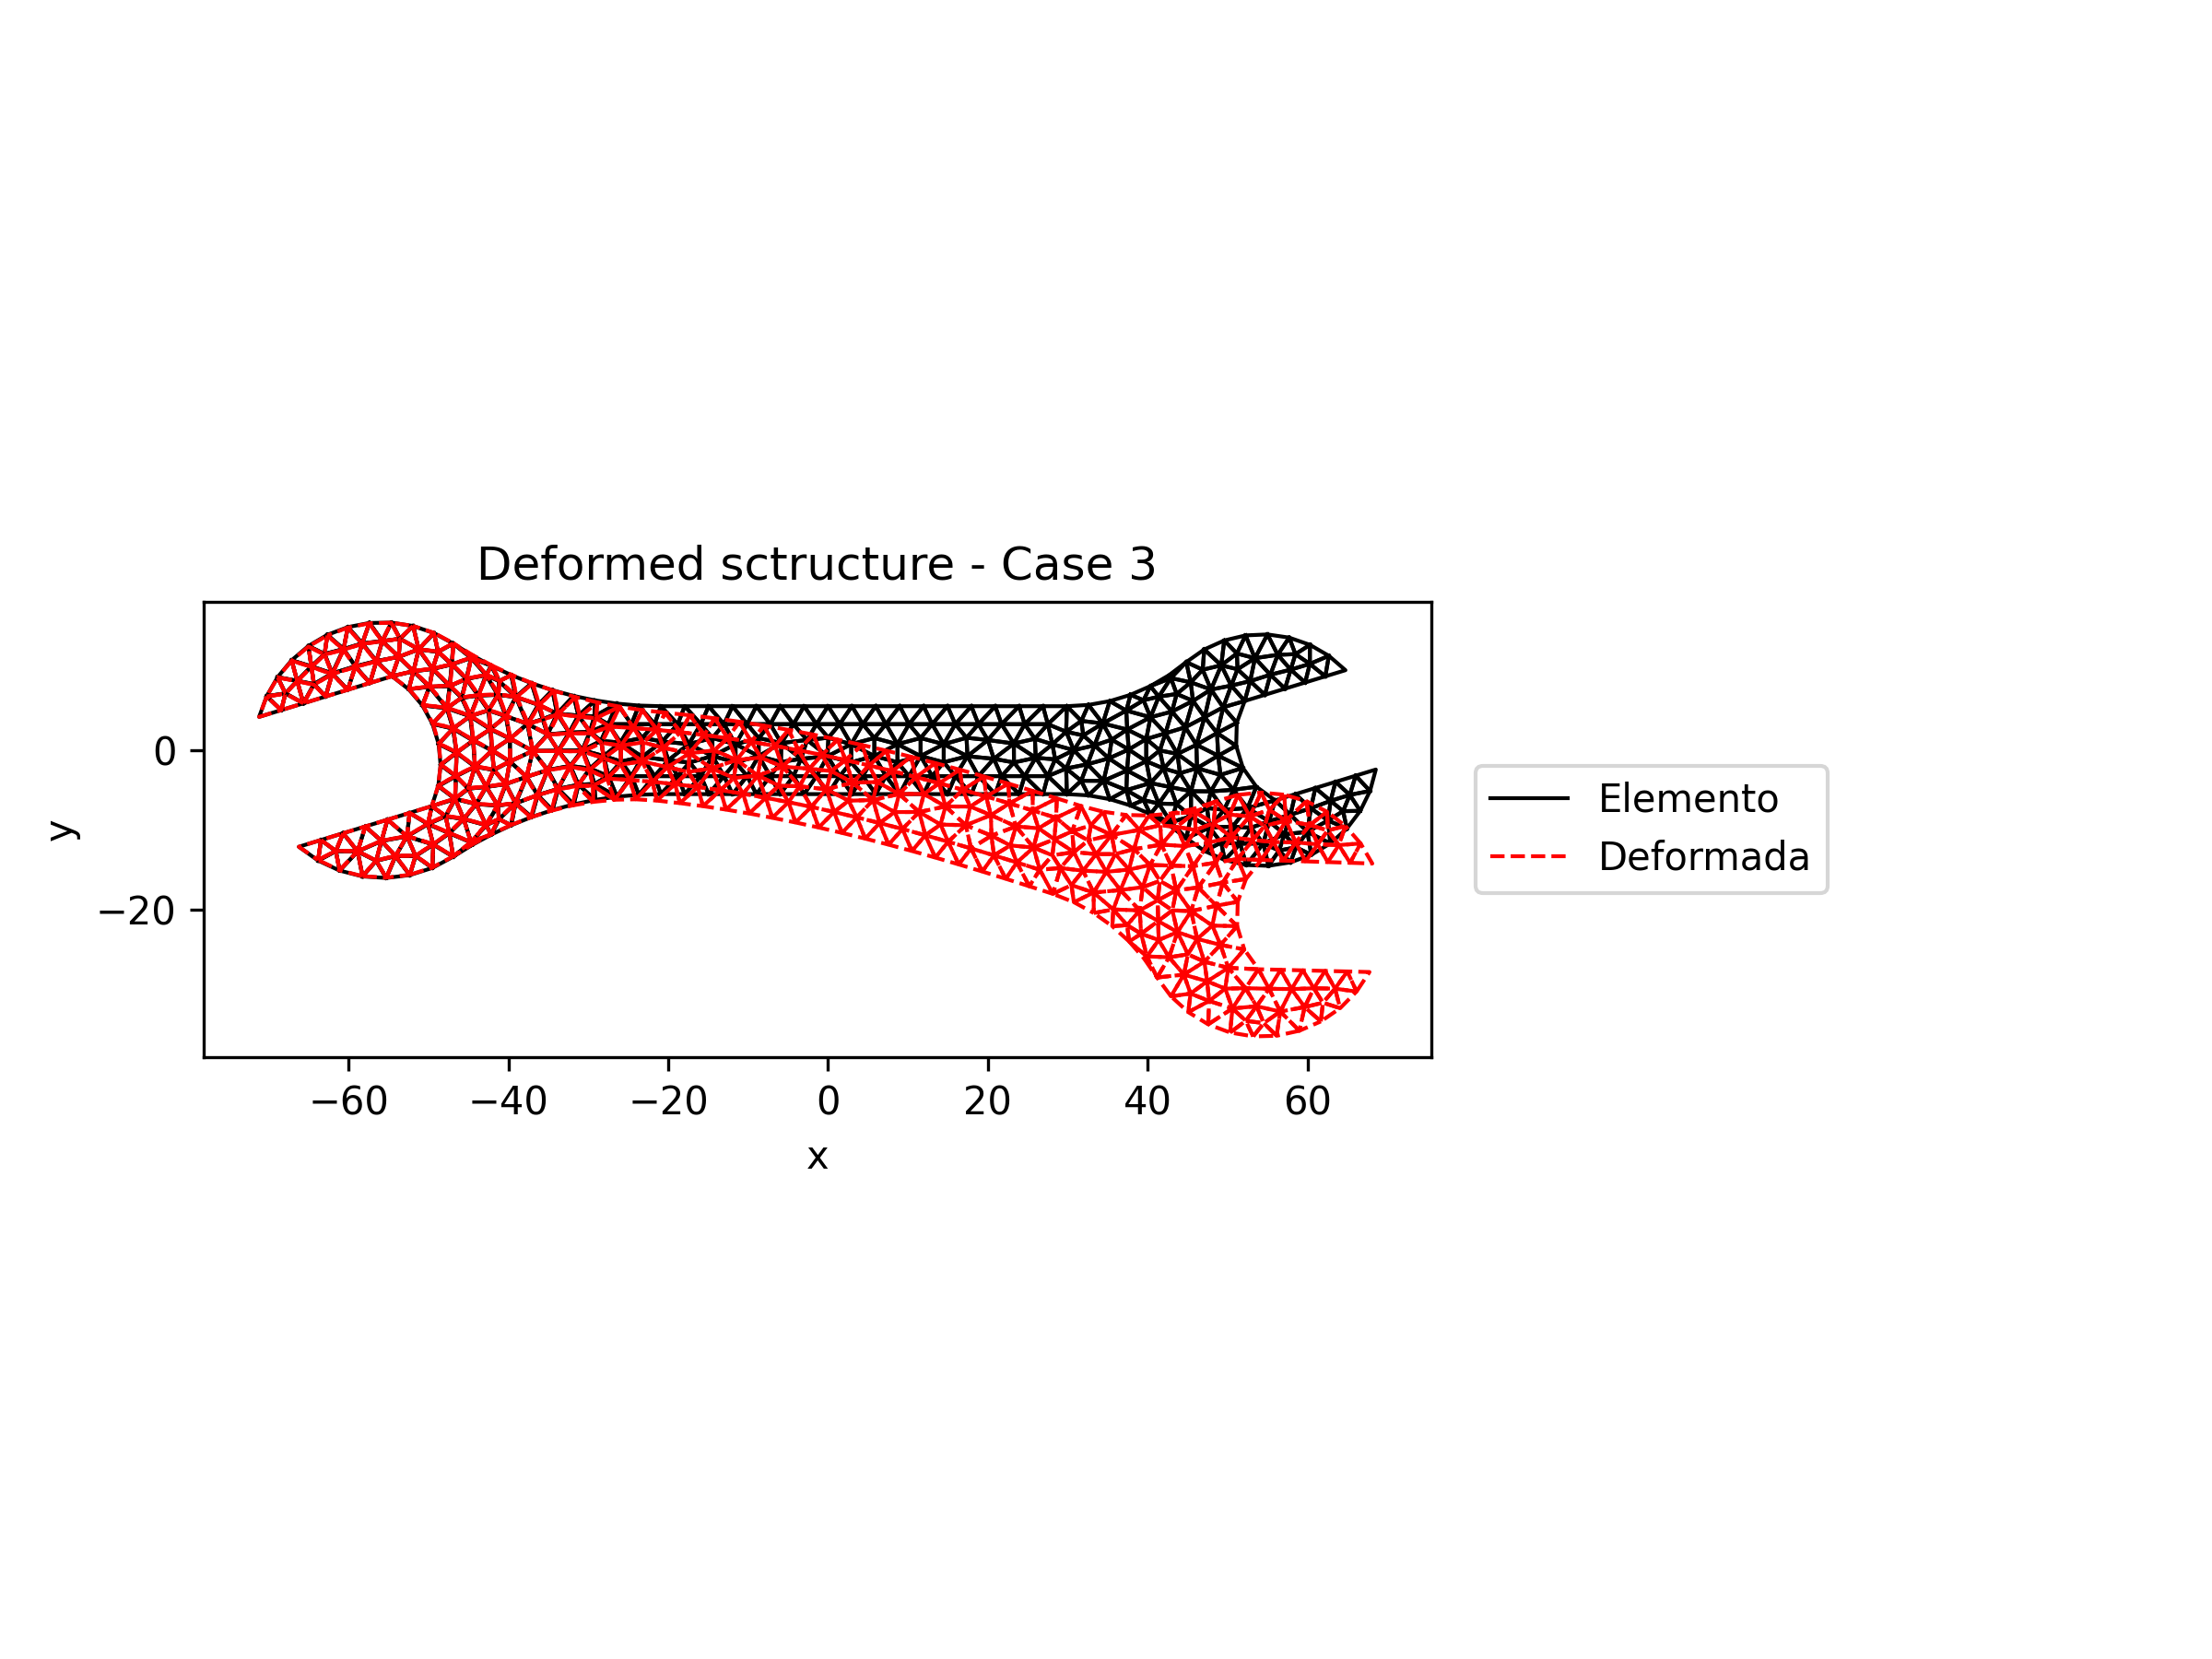
\includegraphics[width=0.8\textwidth]{Resultados/Deformed_sctructure_-_Case_3.png}
    \caption{Deformed structure - Case 3}
    \label{fig:fig23}
\end{figure}

% Imágenes de a dos:
\begin{figure}[H]
    \centering
    \begin{minipage}{0.48\textwidth}
        \centering
        \includegraphics[width=\textwidth]{Resultados/Case_3_-_Maximum_Principal_Stress_σ1.png}
        \caption{Maximum Principal Stress $\sigma_1$}
        \label{fig:fig24}
    \end{minipage}
    \hfill
    \begin{minipage}{0.48\textwidth}
        \centering
        \includegraphics[width=\textwidth]{Resultados/Case_3_-_Minimum_Principal_Strain_ε2.png}
        \caption{Minimum Principal Strain $\epsilon_2$}
        \label{fig:fig25}
    \end{minipage}
\end{figure}

\begin{figure}[H]
    \centering
    \begin{minipage}{0.48\textwidth}
        \centering
        \includegraphics[width=\textwidth]{Resultados/Case_3_-_Strain_εxx.png}
        \caption{Strain $\epsilon_{xx}$}
        \label{fig:fig26}
    \end{minipage}
    \hfill
    \begin{minipage}{0.48\textwidth}
        \centering
        \includegraphics[width=\textwidth]{Resultados/Case_3_-_Strain_εxy.png}
        \caption{Strain $\epsilon_{xy}$}
        \label{fig:fig27}
    \end{minipage}
\end{figure}

\begin{figure}[H]
    \centering
    \begin{minipage}{0.48\textwidth}
        \centering
        \includegraphics[width=\textwidth]{Resultados/Case_3_-_Strain_εyy.png}
        \caption{Strain $\epsilon_{yy}$}
        \label{fig:fig28}
    \end{minipage}
    \hfill
    \begin{minipage}{0.48\textwidth}
        \centering
        \includegraphics[width=\textwidth]{Resultados/Case_3_-_Maximum_Principal_Strain_ε1.png}
        \caption{Maximum Principal Strain $\epsilon_1$}
        \label{fig:fig29}
    \end{minipage}
\end{figure}

\begin{figure}[H]
    \centering
    \begin{minipage}{0.48\textwidth}
        \centering
        \includegraphics[width=\textwidth]{Resultados/Case_3_-_Minimum_Principal_Stress_σ2.png}
        \caption{Minimum Principal Stress $\sigma_2$}
        \label{fig:fig30}
    \end{minipage}
    \hfill
    \begin{minipage}{0.48\textwidth}
        \centering
        \includegraphics[width=\textwidth]{Resultados/Case_3_-_Stress_σxx.png}
        \caption{Stress $\sigma_{xx}$}
        \label{fig:fig31}
    \end{minipage}
\end{figure}

\begin{figure}[H]
    \centering
    \begin{minipage}{0.48\textwidth}
        \centering
        \includegraphics[width=\textwidth]{Resultados/Case_3_-_Stress_σxy.png}
        \caption{Stress $\sigma_{xy}$}
        \label{fig:fig32}
    \end{minipage}
    \hfill
    \begin{minipage}{0.48\textwidth}
        \centering
        \includegraphics[width=\textwidth]{Resultados/Case_3_-_Stress_σyy.png}
        \caption{Stress $\sigma_{yy}$}
        \label{fig:fig33}
    \end{minipage}
\end{figure}

\newpage
\section{Questions}

\subsection{¿How do you know convergence in mesh size has been achieved?}

Convergence was verified by analyzing the variation of the results as the mesh was refined.  
The maximum principal stress $\sigma_1$ was monitored for different mesh sizes, and it was observed that as the mesh became finer, the changes in $\sigma_1$ between refinements became smaller.  
Once the variation between two successive meshes was small enough, convergence was considered achieved.

\subsection{¿How do the stress/strain fields look like before and after smoothing?}

Before smoothing, the stress and strain fields show small numerical oscillations and abrupt color changes, especially near areas with high stress gradients or mesh irregularities.  
After applying smoothing, the fields become much more continuous and the contours appear cleaner and more physically realistic, helping to better visualize stress concentrations and deformation patterns.
\\
\begin{figure}[H]
    \centering
    \begin{minipage}{0.48\textwidth}
        \centering
        \includegraphics[width=\textwidth]{Resultados/Case_3_-_Maximum_Principal_Stress_σ1.png}
        \caption{Maximum Principal Stress $\sigma_1$ - Case 3 with high resolution}
        \label{fig:stress_case1_high}
    \end{minipage}
    \hfill
    \begin{minipage}{0.48\textwidth}
        \centering
        \includegraphics[width=\textwidth]{Resultados/Case_low_resolution_3_-_Maximum_Principal_Stress_σ1.png}
        \caption{Maximum Principal Stress $\sigma_1$ - Case 3 with low resolution}
        \label{fig:stress_case3_low}
    \end{minipage}
\end{figure}

\subsection{¿What differences do you see when applying the load as a distributed load vs. a point load?}

When applying the load as a distributed force, the stress and strain fields are smoother and more evenly distributed along the loaded edge.  
In contrast, when the same total load is applied at a single node (point load), the stresses and strains become highly concentrated around that node, producing very sharp gradients and localized deformation.

The distributed load better represents a realistic load application, while the point load generates an idealized, more critical scenario that can artificially amplify local stresses.

\subsection{¿Is it necessary to consider self weight for an accurate analysis of the tool?}

For lightweight tools like a small 3D-printed wrench, the self-weight has a minor effect compared to the external load, slightly increasing the stresses and displacements, mainly towards the free end.

Although the impact is small, including the self-weight leads to a more accurate and complete analysis, especially if precise stress predictions are required or if the tool size and weight are larger.

\begin{figure}[H]
    \centering
    \begin{minipage}{0.48\textwidth}
        \centering
        \includegraphics[width=\textwidth]{Resultados/Case_1_-_Maximum_Principal_Stress_σ1.png}
        \caption{Maximum Principal Stress $\sigma_1$ - Case 1 (without self-weight)}
        \label{fig:stress_case1}
    \end{minipage}
    \hfill
    \begin{minipage}{0.48\textwidth}
        \centering
        \includegraphics[width=\textwidth]{Resultados/Case_3_-_Maximum_Principal_Stress_σ1.png}
        \caption{Maximum Principal Stress $\sigma_1$ - Case 3 (with self-weight)}
        \label{fig:stress_case3}
    \end{minipage}
\end{figure}

Comparing the maximum principal stress fields between Case 1 and Case 3 shows that the overall stress distribution pattern remains similar.  
However, the stress magnitudes are slightly higher in Case 3 due to the additional contribution of the self-weight, especially towards the free end of the wrench.

\subsection{Research or provide a reasonable stress-based failure criteria for PLA. For this loading condition, and based on your failure criteria ¿where do you expect the wrench to fail?}

For PLA, a reasonable failure criterion is to assume failure occurs when the maximum principal stress $\sigma_1$ exceeds approximately 50 MPa, which is a conservative estimate for 3D-printed materials.

Based on the stress distribution obtained from the analysis, the highest $\sigma_1$ values are located near the section changes of the wrench.  
Therefore, failure is expected to initiate in that region due to the high concentration of stresses.


\section{Optimization of the Design to Reduce Maximum Stress}

For this stage, a mesh with element size $3$ was selected, providing a good balance between computational cost and solution accuracy based on the previous mesh convergence study.

The goal was to minimize the maximum principal tensile stress $\sigma_1$ while keeping the total volume of material constant.  
To achieve this, the geometry of the wrench was modified by redistributing $50\%$ of material from the head to the handle.
Specifically, the thickness of the handle was increased to unify it more effectively with the body of the wrench, reinforcing the critical connection area where high stress concentrations were observed.  
At the same time, the thickness of the head was slightly reduced, compensating for the material added to the handle and preserving the total volume. At the end of the process, the heads of the wrench ended with 3.54 mmof thickness, while the whole handle was increased to 3.7 mm.

The design process was iterative. The initial stress distribution was analyzed to identify the regions under maximum stress. Based on this information, localized changes to the geometry were proposed and the modified wrench was reanalyzed to verify the stress reduction.  
This process was repeated until a satisfactory decrease in the maximum principal tensile stress was achieved without increasing the material volume.

The final design demonstrated a reduction in the maximum $\sigma_1$ values compared to the original configuration. 
\newpage

\section{Bibliography}

\begin{thebibliography}{9}

\bibitem{wikipediaPLA}
Wikipedia contributors. (no date) \textit{Polylactic acid}. Wikipedia. Available at: \url{https://en.wikipedia.org/wiki/Polylactic_acid} (Accessed: 28 April 2025).
    
\end{thebibliography}
\end{document}

